\documentclass[margin=5mm]{standalone}
\usepackage[T1]{fontenc}
\usepackage[utf8]{inputenc}
\usepackage{pgf,tikz, pgfplots}
\usetikzlibrary{calc}
\usetikzlibrary{intersections}
\pgfplotsset{compat=newest}
\usetikzlibrary{shapes}

\begin{document}

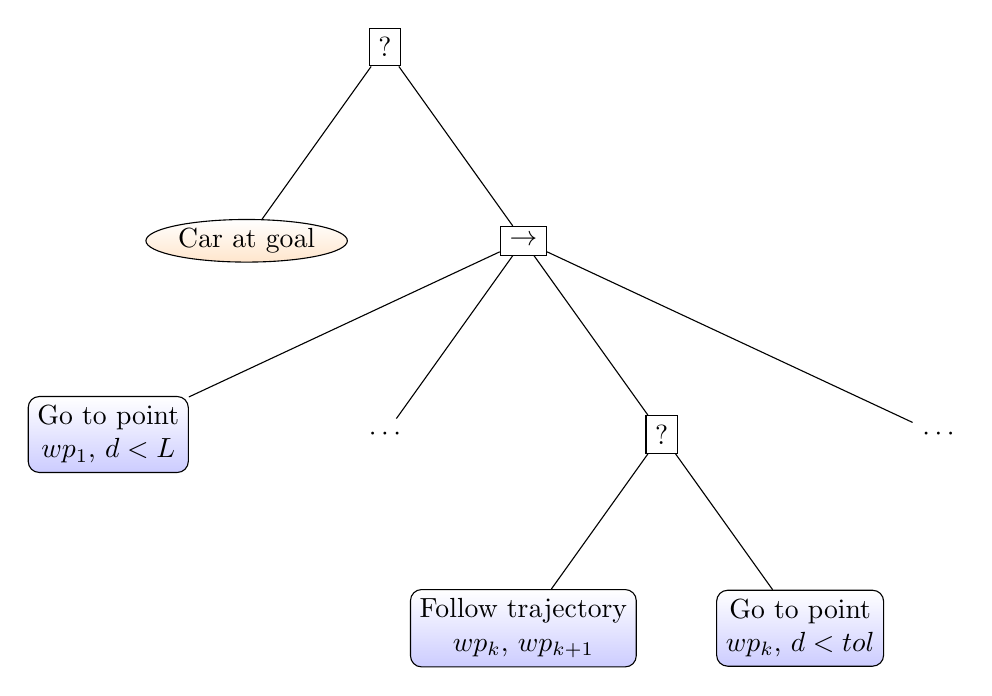
\begin{tikzpicture}[sibling distance=10em, level distance=7em,
  condition/.style = {shape=ellipse, draw, align=center,
    top color=white, bottom color=orange!20, inner sep=1pt},
  sequence/.style = {shape=rectangle, draw,},
  fallback/.style = {shape=rectangle, draw,},
  action/.style = {shape=rectangle, rounded corners,
    draw, align=center,
    top color=white, bottom color=blue!20}]]
  \node[fallback] {?}
  child { node[condition] {Car at goal} }
  child { node[sequence, ] {$\rightarrow$}
    child { node[action] {Go to point\\ $wp_1$, $d<L$} }
    child { node[] {$\cdots$} }
    child { node[fallback] {?}
    child { node[action] {Follow trajectory\\
        $wp_k$, $wp_{k+1}$} }
    child { node[action] {Go to point\\ $wp_k$, $d<tol$} }
  }
  child { node[] {$\cdots$} }
  };
\end{tikzpicture}

\end{document}
